\begin{figure}[htbp]
\centering
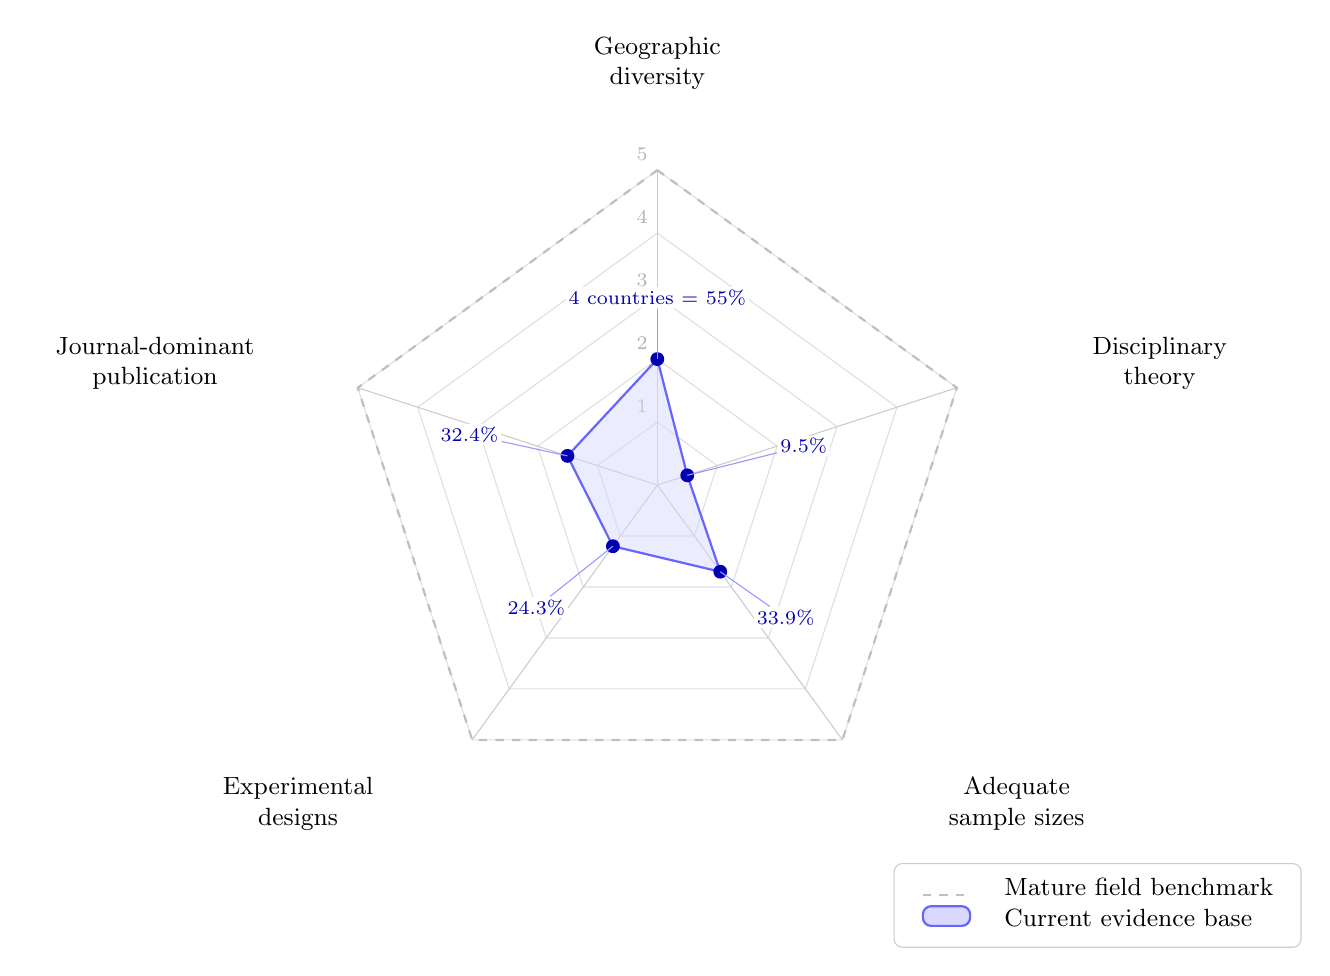
\begin{tikzpicture}

% Pentagon axes — 5 dimensions of evidence maturity
\def\maxrad{4.0}

% Axis labels — positioned well outside the chart
\node[font=\small, text width=3.2cm, align=center, anchor=south] at (90:\maxrad+0.9) {Geographic\\diversity};
\node[font=\small, text width=3cm, align=center, anchor=east] at (162:\maxrad+1.0) {Journal-dominant\\publication};
\node[font=\small, text width=3cm, align=center, anchor=east] at (234:\maxrad+1.0) {Experimental\\designs};
\node[font=\small, text width=3cm, align=center, anchor=west] at (306:\maxrad+1.0) {Adequate\\sample sizes};
\node[font=\small, text width=3cm, align=center, anchor=west] at (18:\maxrad+1.0) {Disciplinary\\theory};

% Grid rings (1-5)
\foreach \r in {1,...,5} {
    \draw[gray!25, thin] (90:\r*\maxrad/5) \foreach \a in {162,234,306,18,90} {-- (\a:\r*\maxrad/5)} -- cycle;
}

% Axis lines
\foreach \a in {90,162,234,306,18} {
    \draw[gray!40, thin] (0,0) -- (\a:\maxrad);
}

% Scale labels on first axis (90°)
\foreach \r/\lab in {1/1, 2/2, 3/3, 4/4, 5/5} {
    \node[font=\scriptsize, text=gray!60, anchor=south east] at (90:\r*\maxrad/5) {\lab};
}

% Ideal mature field (5 on all axes) — dashed outline
\draw[gray!50, dashed, thick]
    (90:\maxrad) --
    (162:\maxrad) --
    (234:\maxrad) --
    (306:\maxrad) --
    (18:\maxrad) -- cycle;

% Actual field status values (out of 5):
% Geographic diversity: 4 countries = 55% → 2/5
% Journal ratio: 32.4% → 1.5/5
% Experimental designs: 24.3% → 1.2/5
% Adequate samples (≥30): 33.9% → 1.7/5
% Disciplinary theory: 9.5% → 0.5/5
\draw[blue!60, thick, fill=blue!15, fill opacity=0.5]
    (90:2*\maxrad/5) --
    (162:1.5*\maxrad/5) --
    (234:1.2*\maxrad/5) --
    (306:1.7*\maxrad/5) --
    (18:0.5*\maxrad/5) -- cycle;

% Data points
\foreach \a/\v in {90/2, 162/1.5, 234/1.2, 306/1.7, 18/0.5} {
    \fill[blue!70!black] (\a:\v*\maxrad/5) circle (2.5pt);
}

% Value annotations — pulled outward with leader lines
% Geographic diversity (top)
\node[font=\scriptsize, text=blue!70!black, anchor=south, fill=white, inner sep=1pt, rounded corners=1pt]
    (geo) at (90:2.8*\maxrad/5) {4 countries = 55\%};
\draw[blue!40, thin] (90:2*\maxrad/5) -- (geo);

% Journal ratio (upper left)
\node[font=\scriptsize, text=blue!70!black, anchor=east, fill=white, inner sep=1pt, rounded corners=1pt]
    (jour) at (162:2.6*\maxrad/5) {32.4\%};
\draw[blue!40, thin] (162:1.5*\maxrad/5) -- (jour);

% Experimental designs (lower left)
\node[font=\scriptsize, text=blue!70!black, anchor=east, fill=white, inner sep=1pt, rounded corners=1pt]
    (exp) at (234:2.4*\maxrad/5) {24.3\%};
\draw[blue!40, thin] (234:1.2*\maxrad/5) -- (exp);

% Adequate samples (lower right)
\node[font=\scriptsize, text=blue!70!black, anchor=west, fill=white, inner sep=1pt, rounded corners=1pt]
    (samp) at (306:2.6*\maxrad/5) {33.9\%};
\draw[blue!40, thin] (306:1.7*\maxrad/5) -- (samp);

% Disciplinary theory (right)
\node[font=\scriptsize, text=blue!70!black, anchor=west, fill=white, inner sep=1pt, rounded corners=1pt]
    (disc) at (18:2.0*\maxrad/5) {9.5\%};
\draw[blue!40, thin] (18:0.5*\maxrad/5) -- (disc);

% Legend (bottom right, outside chart)
\node[draw=gray!40, fill=white, rounded corners=3pt, inner sep=4pt, font=\small,
      anchor=north west] at (3.0, -4.8) {
    \begin{tabular}{ll}
    \tikz\draw[gray!50, dashed, thick] (0,0) -- (0.6,0); & Mature field benchmark \\
    \tikz\fill[blue!15, draw=blue!60, thick] (0,0) rectangle (0.6,0.25); & Current evidence base \\
    \end{tabular}
};

\end{tikzpicture}
\caption{Evidence maturity profile of the gamification-in-history-education corpus across five diagnostic dimensions: the shaded area (actual status) compared to the dashed outline (mature field benchmark) reveals systematic underdevelopment across all dimensions, with disciplinary theory integration showing the largest gap}
\label{fig:evidence-maturity-profile}
\end{figure}
